\documentclass{article}
\usepackage{CJKutf8}
\usepackage{amsmath}
\usepackage{listings}
\usepackage{graphicx}

\usepackage[a4paper, total={6in, 10.5in}]{geometry}

\title{醉酒程式-大一 PA}
\date{May 5, 2023}
\begin{document}
\begin{CJK*}{UTF8}{bsmi}

\maketitle

\section*{車輛管理委員會是國立孫逸仙大學效率最高的行政部門,當然是科學化方式拖吊,以最理性、最ㄐㄅ的方式來拖你們這群猴子的車}

你知道嗎? 國立孫逸仙大學效率最高的行政部門是一個叫車輛管理委員會的部門,是一個對學生的車極為關心的部門,
首先他們有兩組人馬,一組開紅單、一組開拖吊車,早上八點準時出動,一路拖到十一點,中午吃飽睡飽後,
從一點半開始拖到四點半,每年替孫逸仙大學賺進三億新台幣,佔了台灣的GDP 99\%。
你可能會想,怎麼可能這麼好賺,孫逸仙大學的學生們可是身高180智商180的強者,構成了孫逸仙大學這間頂尖大學、全台首府,
古詩說:北台大,南中山,西子灣,東沙島,這些碩士論文都不屑自己寫的學生,怎麼可能被區區的車輛管理委員會抓到呢。
其實車輛管理委員會有開發一項領先世界三億個碩士論文的科技,他們可以將那些違停機車、汽車、直升機、飛機,通通使用
維度轉換,強制壓進一維空間,也就是說,在三維空間排列的物品都會依照他們基於原點的特徵向量,在對其做洛朗展開,
排列進一維空間上的一條線,這樣就可以迅速的收集這些錢錢,阿打錯,是違停。

但即使有這樣一個超級科技,車輛管理委員會還是需要慢慢把那些違停車輛收集到收集車上,但他們希望可以減少拖車的距離,
因為維度展開後,收集車沒辦法移動,所以必須找到一個讓收集車距離所有違停的距離總和最小的地方,你現在被車管會要求寫一個程式幫他們算
以此來換取你的車不會變成他們的人質。\\
此外車管會有個要求,他們希望展開後如果有多個地方都是距離總和最小,就停在位置最小的地方。

以一個簡單的範例來說: 假設現在有$4$個違停在數線上,分別在$1,2,3,4$的位置上,很顯然當收集車停在$2$或$3$的位置上,
對於所有違停的距離總和會最小,這時程式應該要選擇停在$2$而距離總和為$\lvert1-2\rvert+\lvert2-2\rvert+\lvert3-2\rvert+\lvert4-2\rvert=4$。
所以會輸出$2\ 4$。

\begin{figure*}[htb]
    \vspace{-\baselineskip}  
    \begin{center}
        \resizebox{1.0\textwidth}{!}{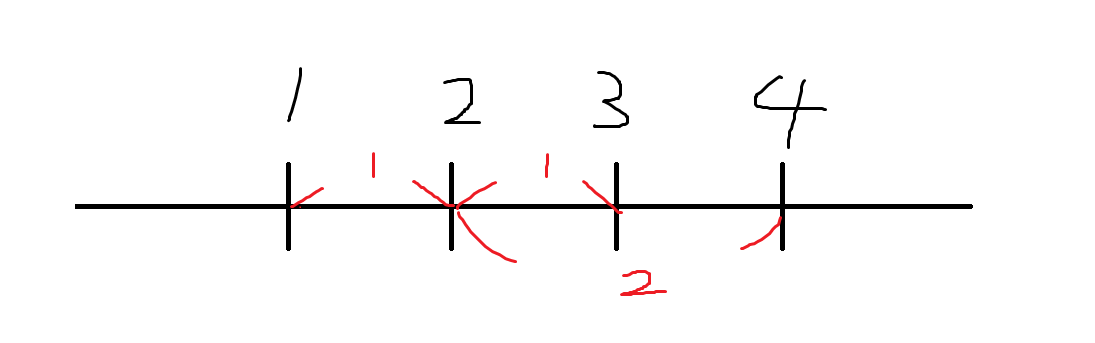
\includegraphics{VMC-example.png}}
      \caption{example}
      \label{fig:example}
    \end{center}
    \vspace{-\baselineskip}
\end{figure*}

\subsection*{輸入格式}
首先會有一個數字$t$,代表接下來有幾組測資。接著會有$t$行,每行都是一組測資,每組測資會包含一個非零正整數$n$,有幾個違停車輛,
接著會有$n$個整數$a_i$,代表那些違停車輛在一維線上的位置。\\
保證$\lvert a_i\rvert <2^{31}$,且保證是由小到大輸入。

\subsection*{輸出格式}
請輸出讓收集車距離所有違停的距離總和最小的位置,接著輸出與所有違停的距離總和,以空白分隔,每個測資的結果請換行。

\subsection*{輸入範例}
$5\\1\ 1\\3\ 1\ 2\ 3\\4\ 1\ 2\ 3\ 4\\5\ 1\ 2\ 3\ 4\ 5\\5\ 4\ 5\ 10\ 7\ 9$

\subsection*{輸出範例}
$1\ 0\\2\ 2\\2\ 4\\3\ 6\\7\ 10$

\subsection*{測資範圍}
\begin{itemize}
    \item testcase 1-3, $t=1,n\leq100$, 占分: $30\%$
    \item testcase 4-6, $t=5,n\leq10^5$, 占分: $30\%$
    \item testcase 7-10, $t=8, n\leq10^6$, 占分: $40\%$
\end{itemize}

\end{CJK*}
\end{document}